%%%%%%%%%%%%%%%%%%%%%%%%%%%%%%%%%%%%%%%%%%%%%%%%%%%%%%%%%%%%%%%%%%%%%%%%%%%%%%%%%%%%%%%%µ%%%%%%%%%%%%%%%%%%
%%%  The State of Linked Data - An Extensible Framework to Validate and Build Dataset Profiles            %%%%
%%%%%%%%%%%%%%%%%%%%%%%%%%%%%%%%%%%%%%%%%%%%%%%%%%%%%%%%%%%%%%%%%%%%%%%%%%%%%%%%%%%%%%%%%%%%%%%%%%%%%%%%%%%

\documentclass[runningheads,a4paper]{llncs}

\usepackage[utf8]{inputenc}
\usepackage{amssymb}
\setcounter{tocdepth}{3}
\usepackage{graphicx}
\usepackage{tabularx}
\usepackage{url}
\usepackage{listings}
\usepackage{subfigure}
\usepackage{algorithmic}
\usepackage{algorithm}

\graphicspath{ {figures/} }

\newcommand{\keywords}[1]{\par\addvspace\baselineskip
\noindent\keywordname\enspace\ignorespaces#1}

% todo macro
\usepackage{color}
\newtheorem{deflda}{Axiom}
\newcommand{\todo}[1]{\noindent\textcolor{red}{{\bf \{TODO}: #1{\bf \}}}}

% Language Definitions for Turtle
\definecolor{olivegreen}{rgb}{0.2,0.8,0.5}
\definecolor{grey}{rgb}{0.5,0.5,0.5}
\lstdefinelanguage{ttl}{
sensitive=true,
morecomment=[l][\color{brown}]{@},
morecomment=[l][\color{red}]{\#},
morestring=[b][\color{blue}]\",
}

%%%%%%%%%%%%%%%%%%%%%%%%%%%%%%%
%%%  Beginning of document  %%%
%%%%%%%%%%%%%%%%%%%%%%%%%%%%%%%

\begin{document}

% first the title is needed
\title{An Extensible Framework to Validate and Build Dataset Profiles}

\author{Ahmad Assaf\inst{1}\inst{2}, Aline Senart\inst{2} and Rapha\"{e}l Troncy\inst{1} }

\institute{EURECOM, Sophia Antipolis, France. \email{<firstName.lastName@eurecom.fr>}
  \and SAP Labs France. \email{<firstName.lastName@sap.com>}
}

% a short form should be given in case it is too long for the running head
\titlerunning{An Extensible Framework to Validate and Build Dataset Profiles}
%\authorrunning{Assaf, Senart and Troncy}

\maketitle

%%%%%%%%%%%%%%%%%%
%%%  Abstract  %%%
%%%%%%%%%%%%%%%%%%

\begin{abstract}
Linked Open Data (LOD) has emerged as one of the largest collection of interlinked datasets on the web. Benefiting from this mine of data requires the existence of descriptive information about each dataset in the accompanying metadata. Such meta information is currently very limited to few data portals where they are usually provided manually thus giving little or bad quality insights. To address this issue, we propose a scalable automatic approach for extracting, validating and generating descriptive linked dataset profiles. This approach applies several techniques to check the validity of the attached metadata as well as providing descriptive and statistical information of a certain dataset as well as a whole data portal. Using our framework on prominent data portals shows that the general state of the Linked Open Data needs attention as most of datasets suffer from bad quality metadata and lack additional informative metrics.
\keywords{Linked Data, Dataset Profile, Metadata, Data Quality}
\end{abstract}

%%%%%%%%%%%%%%%%%%%%%%%%%
%%%  1. Introduction  %%%
%%%%%%%%%%%%%%%%%%%%%%%%%

\section{Introduction}
\label{sec:introduction}
In the last few years the Semantic Web gained a momentum supported by the introduction of many related initiatives like the Linked Open Data (LOD) \cite{BizerHeath2009}. From 12 datasets cataloged in 2007, the Linked Open Data has grown to almost 1000 datasets containing almost 82 billion triples\footnote{http://datahub.io/dataset?tags=lod}. Data is being published by both public and private sectors and covers a diverse set of domains from life sciences to military.

The Linked Open Data is a gold mine for organizations and individuals who are trying to leverage external data sources in order to produce more informed business decisions \cite{Boyd2011}. This success lies in the cooperation between data publishers and consumers. Consumers are empowered to find, share and combine information in their applications easily. However, the heterogeneous nature of data sources reflects directly on the data quality as these sources often contain inconsistent as well as misinterpreted and incomplete information and meta information. Accompanied with the significant variation in size, used languages and freshness, finding useful datasets without prior knowledge is increasingly complicated. This can be clearly noticed in the LOD Cloud \footnote{http://lod-cloud.net} as few datasets like DBPedia \cite{Bizer:2009:DCP:1640541.1640848}, Freebase \cite{Bollacker:2008:FCC:1376616.1376746} and YAGO \cite{Suchanek:2007:YCS:1242572.1242667} are favored over hidden gems that may include domain specific knowledge more suitable for the tasks on hand.

The main entry point for discovering and identifying needed datasets is through public data portals like DataHub\footnote{http://datahub.io} and Europe's Public Data\footnote{http://publicdata.eu} or private ones like Quandl\footnote{https://quandl.com/} and Engima\footnote{http://enigma.io/}. Private portals harness manually curated data from various sources and expose them to users either freely or through paid plans. The data available is of higher quality but lesser quantity compared to what is available in public portals. Similarly in some public data portals, administrators manually review datasets information and attach suitable meta information. This information is mainly in form of predefined tags such as \textit{media, geography, life sciences, etc.} for organization and clustering purposes.
However the increasing number of available datasets makes the review and curation process unsustainable even when outsourced to communities. Furthermore, the diversity of those datasets makes it hard to classify them with a fixed number of predefined tags that can be subjectively assigned without capturing the essence and breadth of the dataset \cite{6690016}.

\textit{Data profiling} is the process of creating descriptive information about the data examined. It is a cardinal activity when facing an unfamiliar dataset \cite{semwebprofiling}.It helps in assessing the importance of the dataset, improving users' ability to search and reuse part of the dataset and detect irregularities to improve its quality. Data profiling typically includes several tasks:
\begin{itemize}
  \item \textbf{Metadata profiling}: Provides general information on the dataset (dataset description, release and update dates, etc.), legal information (license information, openness, etc.), practical information (access points, data dumps, etc.), etc.
  \item \textbf{Statistical profiling}: Provides statistical information about data types and patterns in the dataset, i.e. properties distribution, number of entities and RDF triples, etc.
  \item \textbf{Topical profiling}: Provides descriptive knowledge on the dataset content and structure. This can be in form of tags and categories used to facilitate search and reuse.
\end{itemize}

In this work, we address the above mentioned challenges of automatic validation and generation of descriptive datasets profiles. This paper proposes an extensible framework consisting of a processing pipeline that combines techniques for data portals identification, datasets crawling and a set of pluggable modules combining several profiling tasks. The framework validates the provided dataset metadata against an aggregated standard set of information. Metadata fields are automatically corrected when possible i.e. missing license link. Moreover, a report is created with issues that cannot be automatically fixed and is sent to the dataset's maintainer via e-mail. There exist various statistical and topical profiling tools for both relational and Linked Data. The architecture of the framework allows to easily add them as additional profiling tasks. For this paper, we will focus on Linked Data profiling tools as we will present our findings on the overall state of Linked Data in some of the prominent data portals.

The remainder of the paper is structured as follows. Section 2 reviews related literature. Section 3 describes the framework's architecture to validate and generate dataset profiles. Section 4 shows the results of running this tool on some of the most prominent data portals and analyzes them. Finally, Section 5 presents the conclusion and future work.

%%%%%%%%%%%%%%%%%%%%%%%%%
%%%  2. Related Work  %%%
%%%%%%%%%%%%%%%%%%%%%%%%%

\section{Related Work}
\label{sec:Related Work}

There exists a considerable amount of tools that tackle specific profiling tasks. However, to the best of our knowledge, this is the first effort towards extensible automatic assessment and generation of descriptive dataset profiles. For this paper, we will focus on Linked Data profiling tasks. However, one of the advantages of this framework is the ability to easily configure additional profiling tasks accommodating different data types e.g. relational.\\

\textbf{Metadata profiling}: Data Catalog Vocabulary (DCAT) \cite{Erickson:14:DCV} and the Vocabulary of Interlinked Datasets (VoID) \cite{Cyganiak:11:DLD} are concerned with metadata about RDF datasets. There exists several tools aiming at exposing dataset metadata using these vocabularies. In \cite{BoHm:2011:CVD:2030805.2031001} authors generate VoID descriptions limited to a subset of properties that can be automatically deduced from resources within the dataset. However, it still provides data consumers with interesting insights. Quality Assessment of Data Sources (Flemming's Data Quality Assessment Tool)\footnote{http://linkeddata.informatik.hu-berlin.de/LDSrcAss/datenquelle.php} provides basic metadata assessment as it calculates data quality scores based on manual user input. The user should assign weights to the predefined quality metrics and answer a series of questions regarding the dataset. These include, for example, the use of obsolete classes and properties by defining the number of described entities that are assigned disjoint classes, the usage of stable URIs and whether the publisher provides a mailing list for the dataset. The ODI certificate\footnote {https://certificates.theodi.org/} on the other hand provides a description of the published data quality in plain English. It aspires to act as a mark of approval that helps publishers understand how to publish good open data and users how to use it. It gives publishers the ability to provide assurance and support on their data while encouraging further improvements through an ascending scale. ODI comes as an online and free questionnaire for data publishers focusing on certain characteristics about their data. Although these approaches try to perform metadata profiling, they are either incomplete or manual. In our framework, we propose a more automatized and complete approach.\\

\textbf{Statistical profiling}: Calculating statistical information on datasets is vital to applications dealing with query optimization and answering, data cleansing, schema induction and data mining \cite{profilingWebOfData} \cite{datafinland2} \cite{6690016}. Semantic sitemaps \cite{Cyganiak:2008:SSE:1789394.1789457} and RDFStats \cite{Langegger:2009:RER:1674635.1674691} where one of the first to deal with RDF data statistics and summaries. ExpLOD \cite{Khatchadourian:2010:ESE:2155278.2155300} creates statistics on the interlinking between datasets based on \texttt{owl:sameAs} links. In \cite{semwebprofiling} the author introduces a tool that induces the actual schema of the data and gather corresponding statistics accordingly. LODStats  \cite{Auer:2012:LEF:2413941.2413982} is a stream-based approach that calculates more general dataset statistics. ProLOD++ \cite{6816740} is a Web-based tool that allows LOD analysis via automatically computed hierarchical clustering \cite{5452762}. Aether \cite{makela-aether-2014} generates VoID statistical descriptions of RDF datasets. It also provides a Web interface to view and compare VoID descriptions. LODOP \cite{forchhammer_profiles_2014} is a MapReduce framework to compute, optimize and benchmark dataset profiles. The main target for this framework is to optimize the runtime costs for Linked Data profiling. In \cite{DyLDO} authors calculate certain statistical information for the purpose of observing the dynamic changes in datasets.\\

\textbf{Topical Profiling}: Topical and categorical information facilitates dataset search and reuse. Topical profiling focuses on content-wise analysis at the instances and ontological levels. GERBIL \cite{gerbil} is a general entity annotation framework that provides machine processable output allowing efficient querying. In addition, there exist several entity annotation tools and frameworks \cite{Cornolti:2013:FBE:2488388.2488411} but none of those systems are designed specifically for dataset annotation. In \cite{datafinalnd}, authors created a semantic portal to manually annotate and publish metadata about both LOD and non-RDF datasets. In \cite{6690016}, authors automatically assigned Freebase domains to extracted instance labels of some of the LOD Cloud datasets. The goal was to provide automatic domain identification, thus enabling improving datasets clustering and categorization. In \cite{Bohm:2012:LTG:2396761.2398718}, authors extracted dataset topics by exploiting the graph structure and ontological information, thus removing the dependency on textual labels. In  \cite{scalableApproach} authors generate VoID and VoL\footnote{http://data.linkededucation.org/vol }descriptions via a processing pipeline that extracts dataset topic models ranked on graphical models of selected DBpedia categories.\\

Although the above mentioned tools are able to provide general, statistical and topical information about a dataset, there exist no approach that is able to combine them into a unified profile presented to consumers. Dataset search can be done without relying on attached metadata (tags and categories). For example, there exist several approaches to create LOD indexes. In \cite{Alexander:LDOW09}, authors used VoID descriptions to optimize query processing by determining relevant query-able datasets. In \cite{Harth:2010:DSO:1772690.1772733}, authors created an approximate index structure (QTree) and an algorithm for answering conjunctive queries over Linked Data. SchemEX \cite{Konrath:2012:SEC:2399444.2399563} is a stream-based approach leveraging type and property information of RDF instances to create schema-level indexes.\\
Semantic search engines like Sindice \cite{Delbru2010a}, Swoogle \cite{Ding2004} and Watson \cite{d'Aquin:2011:WMS:2019470.2019476} help in entities lookup but are not designed specifically for dataset search. In \cite{whatShou]ldILinkTo}, authors utilized the sig.ma index \cite{Tummarello10sig.ma:live} to identify appropriate data sources for interlinking.

%%%%%%%%%%%%%%%%%%%%%%%%%
%%%  3. Profiling data portals  %%%
%%%%%%%%%%%%%%%%%%%%%%%%%

\section{Profiling Data Portals}
\label{sec:profiling data portals}

In this section, we provide an overview of the processing steps for validating and generating dataset profiles. Figure 1 shows the main steps which are the following: (i) Data portal identification; (ii) metadata extraction; (iii) instance and resource extraction; (iv) profile validation and generation (v) report generation.

Our framework is built as a Command Line Interface (CLI) application using Node.js\footnote{http://nodejs.org/}. Related functions are encapsulated into modules that can be easily plugged in/out the processing pipeline. The various steps are explained in details below.

\begin{figure}[h!]
  \centering
    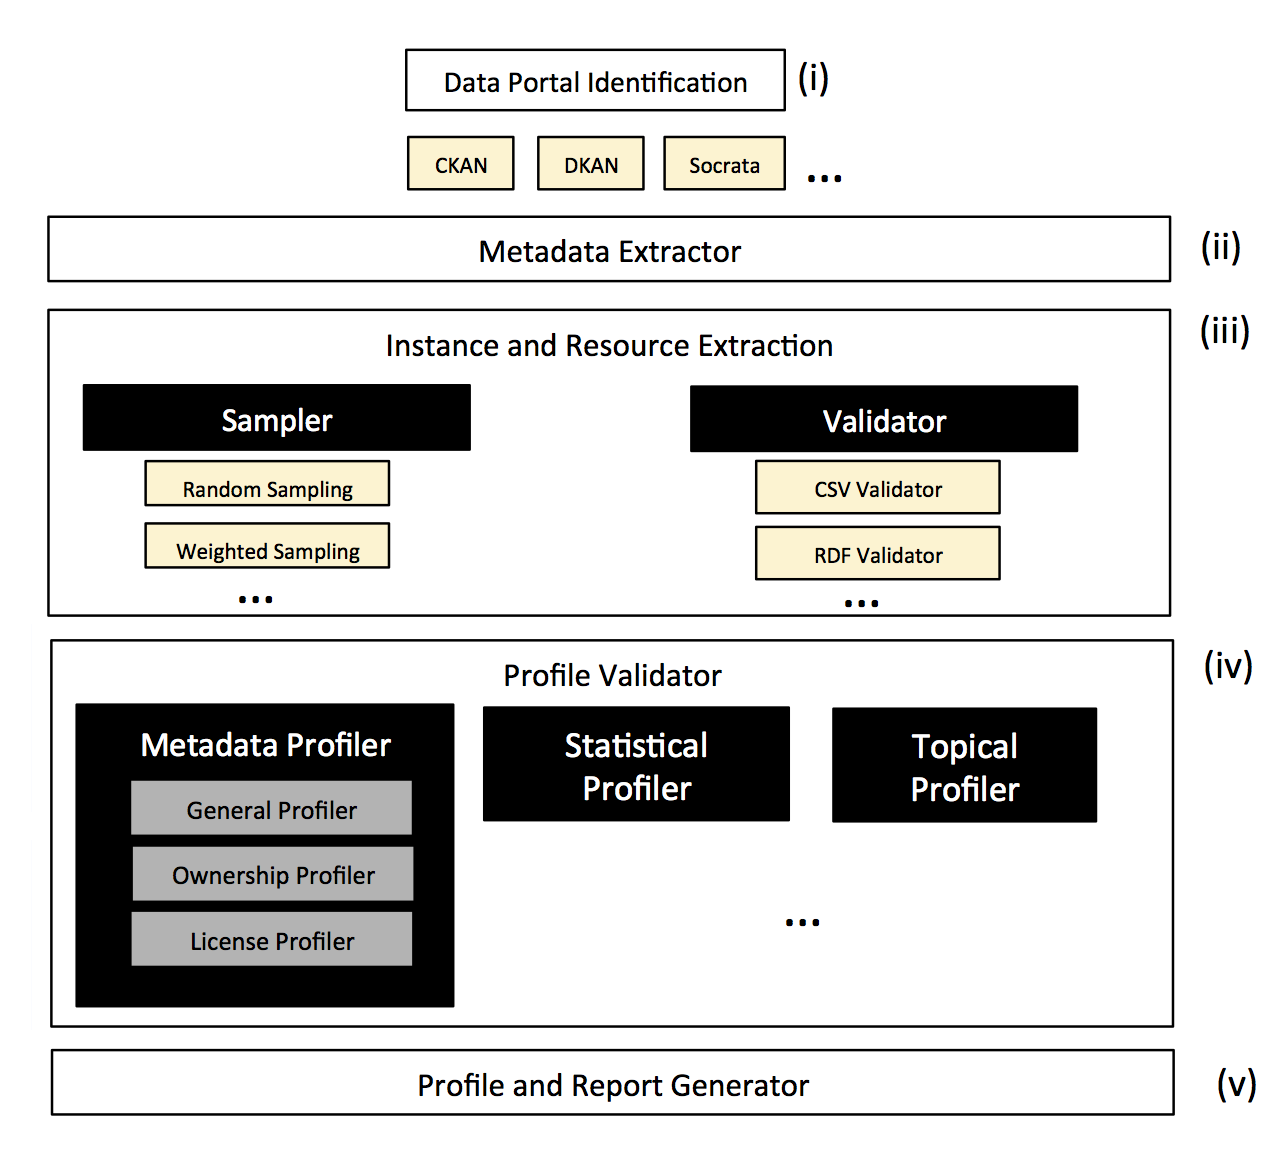
\includegraphics[scale=0.4]{figure-1_architecture.png}
  \caption{Processing pipeline for validating and generating dataset profiles}
\end{figure}

\subsection{Data Portal Identification}

Data portals can be considered as data access points that provide tools facilitating data publishing, sharing, searching and visualization. CKAN\footnote{http://ckan.org} is the world's leading open-source data portal platform powering websites like the DataHub, Europe's Public Data and the U.S Government's open data\footnote{http://data.gov}. Modeled on CKAN, DKAN\footnote{http://drupal.org/project/dkan} is a standalone Drupal distribution that is used in various public data portals as well. Socrata\footnote{http://www.socrata.com} helps public sector organizations improve data-driven decision making by providing a set of solutions including an open data portal. In addition to these tradition data portals, there is a set of tools that allow exposing data directly as RESTful APIs like Datatank\footnote{http://thedatatank.com}, Database-to-API\footnote{https://github.com/project-open-data/db-to-api} and CSV-to-API\footnote{https://github.com/project-open-data/csv-to-api}.\\

Identifying the underline software powering the data portal is a vital first step to understand the API calls needed for the following steps. The identification process can include a combination of the following:

\begin{itemize}
  \item \textbf{URL inspection}: Checking the existence of certain strings in the URL. For example, various CKAN based portals are hosted on subdomains of the \texttt{http://ckan.net} like CKAN Brazil\footnote{http://br.ckan.net} and CKAN Italia\footnote{http://it.ckan.net}.
  \item \textbf{Meta tags inspection}: The \texttt{<meta>} tag provides metadata about the HTML document. They are typically used to specify page description, keywords, author, etc. Inspecting the \texttt{content} attribute can indicate the type of the data portal. For example, \texttt{meta[content*="ckan]} CSS selector can identify CKAN portals, where the \texttt{meta[content*="Drupal"]} can identify DKAN portals.
  \item \textbf{Scripts inspection}: Checking the existence of certain injected or inline JavaScript scripts.
\end{itemize}

After those preliminary checks, we query one of the identified portal API endpoints. The successful completion of the request denotes a successful identification of the data portal type.

\subsection{Metadata Extraction}

After identifying the underlying portal software, we perform iterative queries to the API in order to fetch datasets metadata and persist them in a file-based cache system. Depending on the portal software we can issue specific extraction jobs. For example, in CKAN based portals, we are able to crawl and extract the metadata of a specific dataset, all the datasets in a specific group e.g. LOD Cloud or all the datasets in the portal. Overwriting cached metadata can be done easily by providing custom parameters to the extractor.

\subsection{Instance and Resource Extraction}

From the extracted metadata we are able to identify all the resources associated with that dataset. They can have various types like SPARQL endpoint, API, file, visualization ,etc. Before extracting instance values we do the following:

\begin{itemize}
  \item \textbf{Resource metadata validation}: Check the resource attached metadata values. The metadata should include information about the mimetype, name, description, format, valid de-referenceable URL, size, type and provenance information. The validation process automatically fills up various missing information when possible, like the mimetype and size. However, missing fields like name and description that needs manual input are marked as missing and will appear in the generated summary report.
  \item \textbf{Format validation}: Validate specific resource formats against a linter or a validator e.g. CSV and RDF validators.
\end{itemize}

Considering that certain dataset contain large amount of resources, a sampler module is able to execute various sample-based strategies:
\begin{itemize}
  \item \textbf{Random Sampling}: Randomly selects resources instances.
  \item \textbf{Weighted Sampling}: Weighs each resources as the ratio of the number of datatype properties used to define a resource over the maximum number of datatype properties over all the datasets resources \cite{scalableApproach}.
  \item \textbf{Resource Centrality Sampling}: Weighs each resource as the ration of the number of resource types used to describe a particular resource divided by the total number of resource types in the dataset. This is specific and important to RDF datasets where important concepts tend to be more structured and linked to other concepts \cite{scalableApproach}.
\end{itemize}

\subsection{Profile Validation and Generation}

\subsection{Report Generation}

\bibliographystyle{abbrv}
\nocite{*}
\bibliography{SOLD}
\end{document}
